\chapter{A view of the EoR window from the HERA-19 commissioning array}
\label{chapter:eor_window_HERA}

As emphasized in Chapter~\ref{chapter:eor_window_paper32img}, it is important to constrain intrinsic and leaked polarized signal for any {\sc hi} EoR experiment. 
The objective of this Chapter was an exploration of eight nights of data from the Hydrogen Epoch of Reionization Array (HERA) 19-element commissioning array, coupled with simulations of the instrument, in order to forecast how much of a problem polarization would pose for this interferometer. These results we reported by \cite{Kohn.18}.
This work also represents the first power spectral analysis from HERA. While not in the realm of an EoR-level integration, we were able to offer some initial expectations for this new instrument's performance in the Fourier domain.

This work is organized as follows: in Section~\ref{sec:hera19_leak} we review the theory behind polarization leakage into unpolarized signal and simulate the effect for a model of HERA. In Section~\ref{sec:hera19_obs} we describe the HERA data that we used, its calibration and reduction to power spectra. We present our results, and discuss the implications for HERA's EoR measurements, in Section~\ref{sec:hera19_results}, and conclude in Section~\ref{sec:hera19_conc}. We assume the cosmological parameters reported by \cite{Planck.16} throughout.

\section{Polarization Leakage Simulations}
\label{sec:hera19_leak}

In Chapter~\ref{chapter:interferometry}, we presented direction dependent and independent ways for polarized power to ``leak'' between visibilities. Direction dependent leakage arises because dipole arm `n' is sensitive to electromagnetic radiation with polarization axis aligned with perpendicular dipole arm `e'. Forming pseudo-Stokes visibilities from those in the instrumental basis,

\begin{equation}
\left(\begin{array}{c}
V^{I}\\
V^{Q}\\
V^{U}\\
V^{V}\end{array} \right)
= \frac{1}{2}
\left( \begin{array}{cccc}
1 & 0 & 0 & 1 \\
1 & 0 & 0 & -1 \\
0 & 1 & 1 & 0 \\
0 & -i & i & 0 \end{array} \right) 
\left(\begin{array}{c}
V^{nn}\\
V^{ne}\\
V^{en}\\
V^{ee}\end{array} \right) .
\label{eq:pseudo-stokes}
\end{equation}
results in each pseudo-Stokes visibility containing a direction-dependent mix of the `true' Stokes parameters on the sky. Using simulations of the HERA feed, faceted parabolic dish and analog signal chain \citep{Fagnoni.16}, we proceeded to simulate pseudo-Stokes visibilities using the polarized formalism in Chapter~\ref{chapter:interferometry} (Figure~\ref{fig:interferometry_Mab} shows the direction-dependent leakage matrices used here). 
We simulated visibilities for the HERA-19 commissioning array, described below, using an \textit{unpolarized} model of the low frequency sky from the Global Sky Model \citep[GSM;]{GSM.08, pygsm, GSM.17} at the appropriate R.A. range to match our observations. Forming power spectra and images from these visibilities allowed for a comparison of our data to a `leakage from Stokes I only' regime. At the low frequencies and large scales probed by HERA, Stokes I is extremely bright compared to the other Stokes parameters (e.g. Chapter~\ref{chapter:astro_rad}, \citet{Kohn.16}), so this regime is realistic for the measurements in question.

In Chapter~\ref{chapter:interferometry}, we also presented a formalism for propagating direction-independent calibration errors into polarization leakage. We did not include calibration errors in our simulations, allowing us to build intuition around power spectrum estimates for a ``perfectly behaving'' instrument.

\section{Observations \& Reduction}
\label{sec:hera19_obs}

In this work we used eight nights of observations from the HERA-19 commissioning array. HERA is a low-frequency interferometer composed of 14\,m-diameter dishes arranged in a close-packed hexagonal array of 14.7\,m spacing. The commissioning array consists of nineteen dishes (see Figure~\ref{fig:hera19_antpos}); HERA is being constructed in staged build-outs, and upon completion will consist of 350 dishes in a fractured hexagon configuration \citep[see][]{Dillon.16, deBoer.17}. A feed cage containing two dipole feeds (recycled from the PAPER array, see \citealt{Parsons.10}), oriented in North-South and East-West directions, is suspended above each dish \citep{Neben.16,Ewall-Wice.16.HERA_Dish,Thyagarajan.16}.

HERA only observes in drift-scan mode. The observations we used were eight nights, from Julian Date (JD) 2457548 to 2457555; LSTs 10.5 -- 23 hr. Drift-scan visibilities were recorded every 10.7 seconds for 1024 evenly-spaced channels across the 100-200\,MHz bandwidth. These data were divided into {\sc miriad} data sets roughly 10 minutes long. A night's observation lasted 12 hours in total (6pm to 6am South African Standard Time; SAST); of these we used the central 10 hours, to avoid the thermal effects of the Sun.

\begin{figure}
\centering
\hspace{-0.5cm}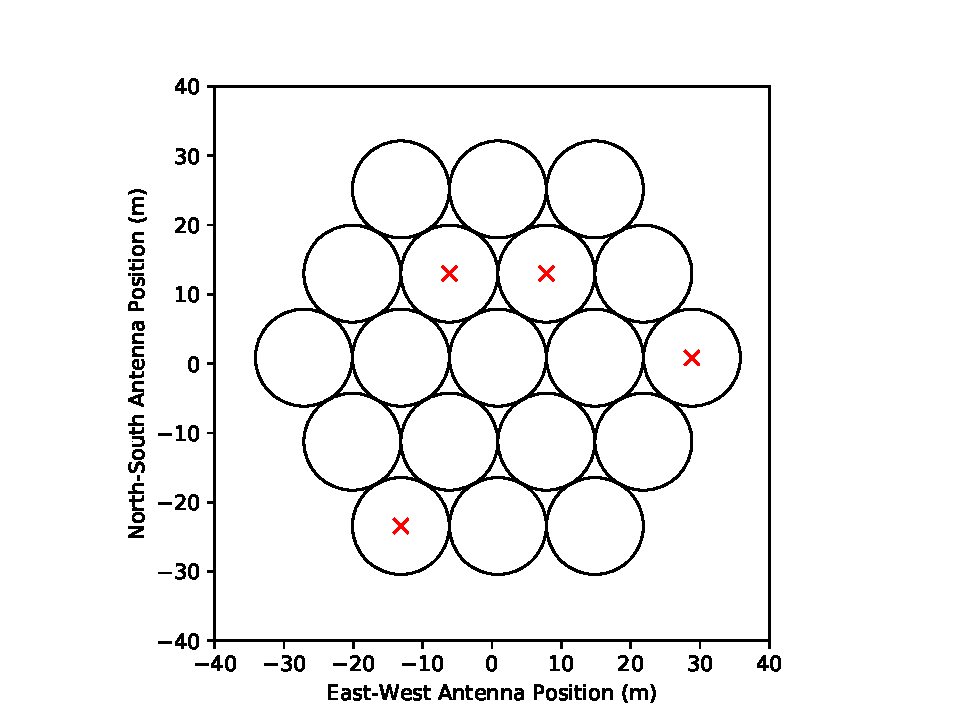
\includegraphics[scale=0.6]{chapters/eor_window_HERA/figures/antpos_hera19.pdf}
\caption[The perimeter of each dish in the HERA-19 array.]{The perimeter of each dish in the HERA-19 array.  A red ``X'' marks antennae that were identified during preprocessing and calibration as malfunctioning and were excluded from further analysis.}
\label{fig:hera19_antpos}
\end{figure}

To identify samples contaminated by radio frequency interference (RFI), a 2D median filter in time and frequency was applied to the visibility data to smooth out high pixel-to-pixel variations, and remove significant outliers that were likely unphysical. The variance of the resulting data was computed, and points with a $z$-score greater than 6 (i.e., points where the value is more than 6$\sigma$ away from the mean) were flagged as initial seeds for RFI extraction. A two-dimensional watershed algorithm was applied using these seeds as starting points, enlarging the regions of RFI-contamination to neighboring pixels with z-scores greater than 2, until all such pixels were flagged. Figure~\ref{fig:hera19_rfi} shows the fractional RFI flag occupancy per time (displayed in LST) and frequency across the 8 days of observations. The majority of the band is relatively clear of RFI. Some clear features are: the FM radio band (below 110 MHz), ORBCOMM satellite communications (137 MHz), an ISS downlink (150 MHz) and VHF TV channels (above 170 MHz)\footnote{For an extended discussion of RFI as seen by HERA, see the public HERA Memo \# 19}.
The Galaxy, when transiting zenith at LST$\approx$17.75 hours, is so bright that it appears to degrade our ability to flag RFI.

\begin{figure}
\centering
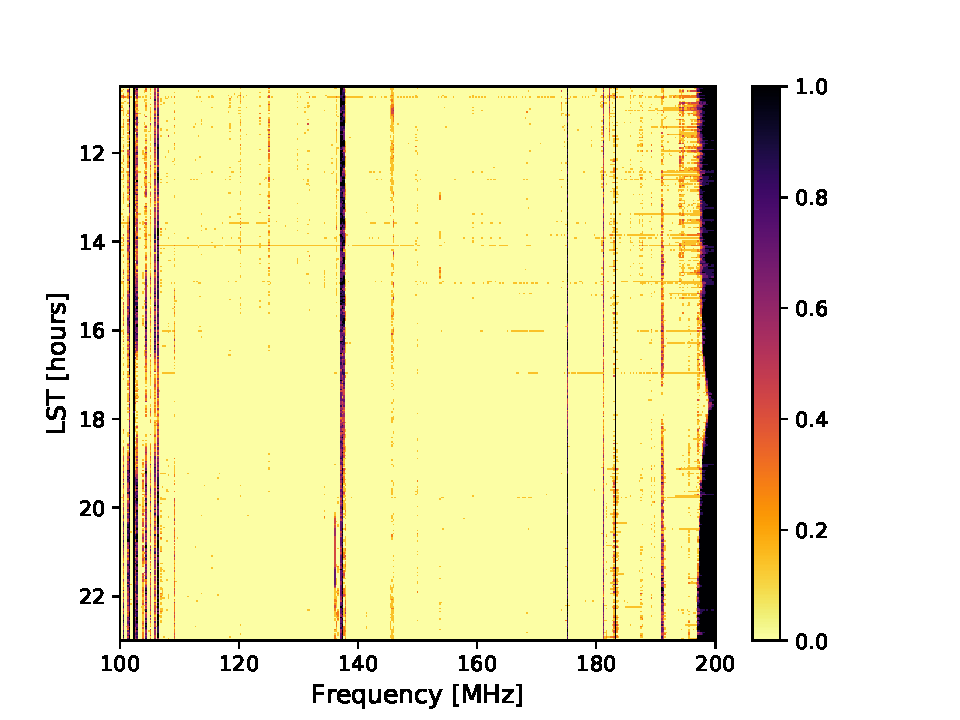
\includegraphics[scale=0.6]{chapters/eor_window_HERA/figures/frac_occ.pdf}
\caption{Fractional RFI flag occupancy per time and frequency over the eight days of observations.}
\label{fig:hera19_rfi}
\end{figure}

\subsection{Calibration}
\label{subsec:hera19_cal}

HERA is designed to be calibrated using redundant calibration techniques \citep{Dillon.16}, but for this preliminary view of HERA commissioning data, we used image-based calibration. Future studies with deeper integrations targeting EoR detections will take advantage of redundancy to obtain more precise calibration solutions \citep{deBoer.17}. We used the {\sc CASA} \citep{casa} package for calibration, taking advantage of its CLEAN, {\tt gaincal} and {\tt bandpass} functions.

To enable the use of {\sc CASA}, we first converted from native {\sc miriad} to a {\sc uvfits} file format which could be ingested by {\sc CASA} using {\sc pyuvdata} \citep{pyuvdata}. 
Using LSTs in which the Galactic center (GC; $\alpha, \delta$ = 17h 45m 40.04s, -29d 0m 28.12s) was transiting, we built a CLEAN model which modeled the GC as an unpolarized point source of strength 1 Jy and flat spectrum, which could be scaled appropriately later (see Equation~\ref{eq:freq_scale}). 
Clearly, this is an incomplete calibration model. However, as the objective of this work is to explore the response of the instrument in power spectrum space without combining baselines of different lengths, most of the purpose of the calibration is correcting an initial large cable delay per antenna. 
Treating the GC as unpolarized is adequate for this study. The large optical depth towards the GC \citep{Oppermann.12} results in large amounts depolarization in the plane of the Galaxy \citep{Wolleben.06}. Moreover, we expected non-negligible amounts of beam depolarization due to the large solid angle of the synthesized beam.

For each night of observations, we used the {\sc CASA} {\tt gaincal} and {\tt bandpass} functions to obtain frequency-dependent phase and amplitude solutions for each antenna and dipole arm. Four antennae had very deviant solutions, and their inclusion resulted in low-quality images. These were omitted from further analysis (and are marked with red ``X''s in Figure~\ref{fig:hera19_antpos}).  Before calibration, we manually flagged the edges of the band (below 110 MHz and above 190 MHz), where spectral behavior is dominated by the high and low pass filtering in the HERA signal chain \citep{deBoer.17}.

In Figure~\ref{fig:hera19_GCimage}, we show images formed from the simulated pseudo-Stokes visibilities (top panels) and our observations (bottom panels). These are multi-frequency synthesis images, where we used all unflagged frequencies on either side of the band edges; 115 MHz to 188 MHz. We do not specify a beam model during imaging. At HERA's position ((latitude, longitude) = (-30:43:17.5, 21:25:41.9)) the Galactic Center transits 2$^{\circ}$ from zenith, while the HERA primary beam has a FWHM of $\sim5^{\circ}$ at 150\,MHz \citep{Neben.16}. For the simulated visibilities, we flagged the same antennae as in the data. As expected for a compact array, the Stokes I images capture only a low-resolution view of the Galactic Center. The simulated and observed visibilities form remarkably similar images in Stokes I, Q and U, but the simulation under-predicts pseudo-Stokes V power. We defer further discussion to Section~\ref{sec:hera19_results}.

\begin{figure*}
\centering
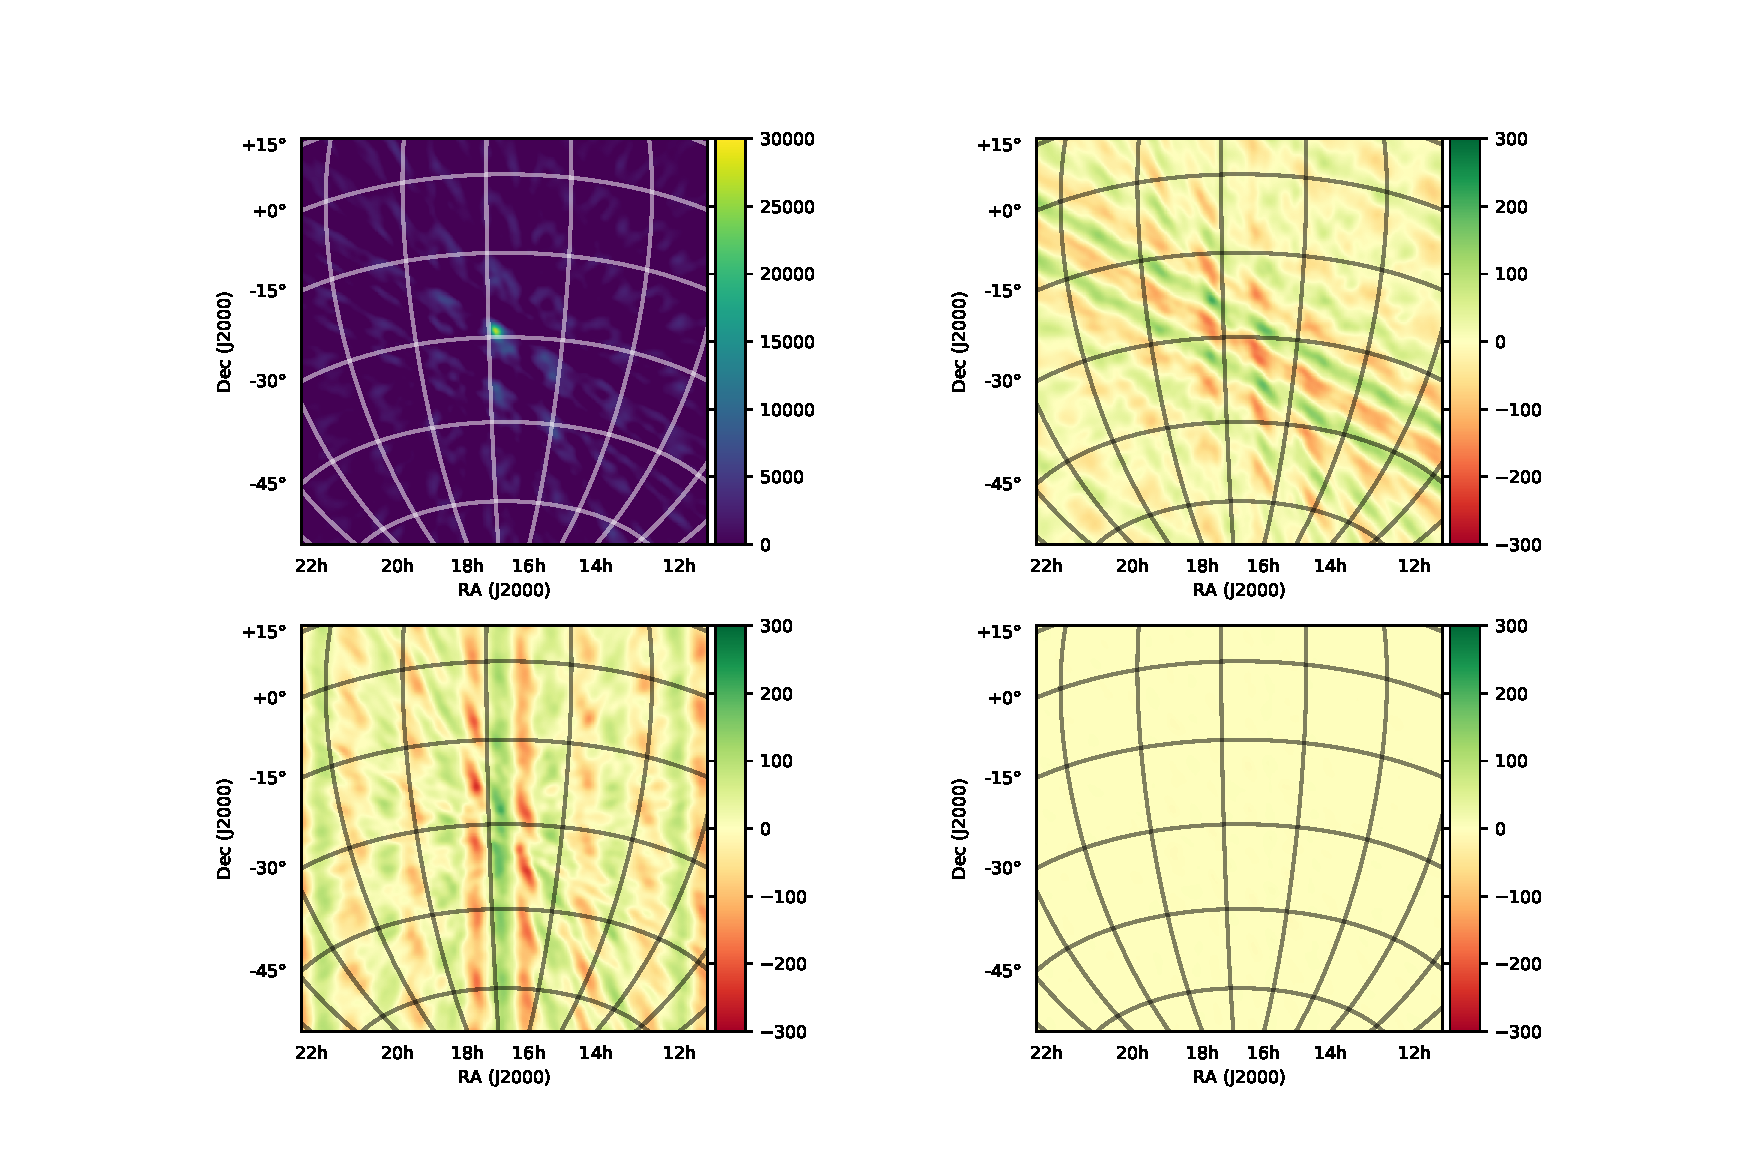
\includegraphics[width=0.7\textwidth]{chapters/eor_window_HERA/figures/sim4pol.pdf}
\par\noindent\rule{0.8\textwidth}{0.4pt}
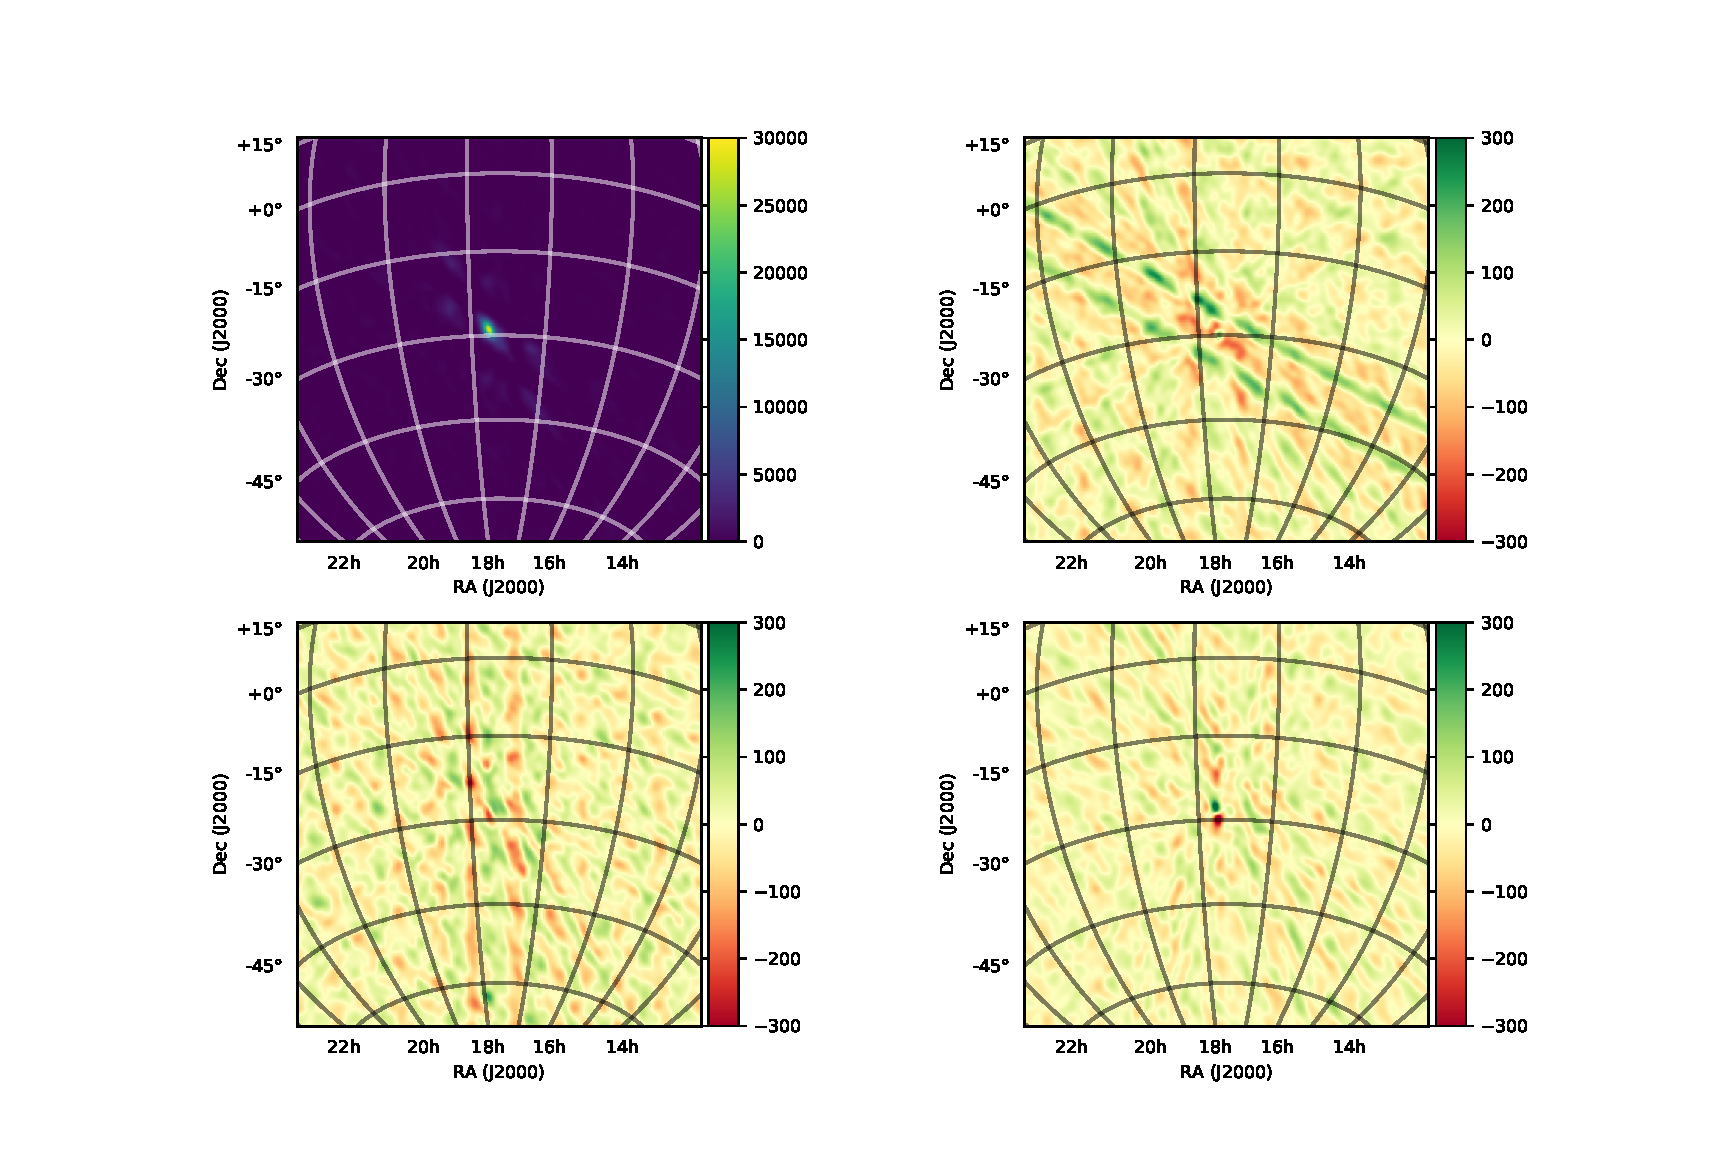
\includegraphics[width=0.7\textwidth]{chapters/eor_window_HERA/figures/new4pol.pdf}
\caption[Multi-frequency synthesis pseudo-Stokes images formed from simulation and data.]{
\textit{Above}: Multi-frequency synthesis pseudo-Stokes images formed from simulation, where only a Stokes I sky was used; any polarized power is due to direction-dependent polarization leakage (see Section~\ref{sec:hera19_leak}).
\textit{Below}: Multi-frequency synthesis pseudo-Stokes images formed from observed visibilities on JD 2457548.
Both sets of panels show the Galactic Center (our calibrator source) close to transit in pseudo-Stokes I, Q, U and V visibilities (\textit{top left, top right, lower left, lower right}). A Briggs-weighting with robustness 0 was used when gridding into the image plane. No deconvolution was performed. The colorbar is in units of Jy/Beam.
A separate color scale is used for Stokes I for suitable dynamic range. An R.A., Dec. grid is shown, illustrating the wide-field nature of HERA observations.
}
%The color scale is normalized to the peak flux of the Galactic Center in Stokes I.} %The excess at the center of the Stokes Q image suggests a $\sim 1\%$ error in the gain solutions, while the excess in Stokes V suggests D-terms at the $\sim 1\%$ level \citep{TMS}.}
\label{fig:hera19_GCimage}
\end{figure*}

Example bandpass solutions from JD 2457548 are shown in Figure~\ref{fig:hera19_bandpass}. Although some residual RFI remains obvious, the derived bandpasses were smooth.  Thus, even though the gains were imprecise, we expected that using them should not add additional spectral structure.  %Spectrally non-smooth gain errors would have the effect of coupling significant amounts foreground signal into the EoR window; see Section \ref{subsec:pspec} below.
% It's not whether the bandpass is smooth, but if *after correcting for the bandpass*, the errors are unsmooth.

\begin{figure}
\centering
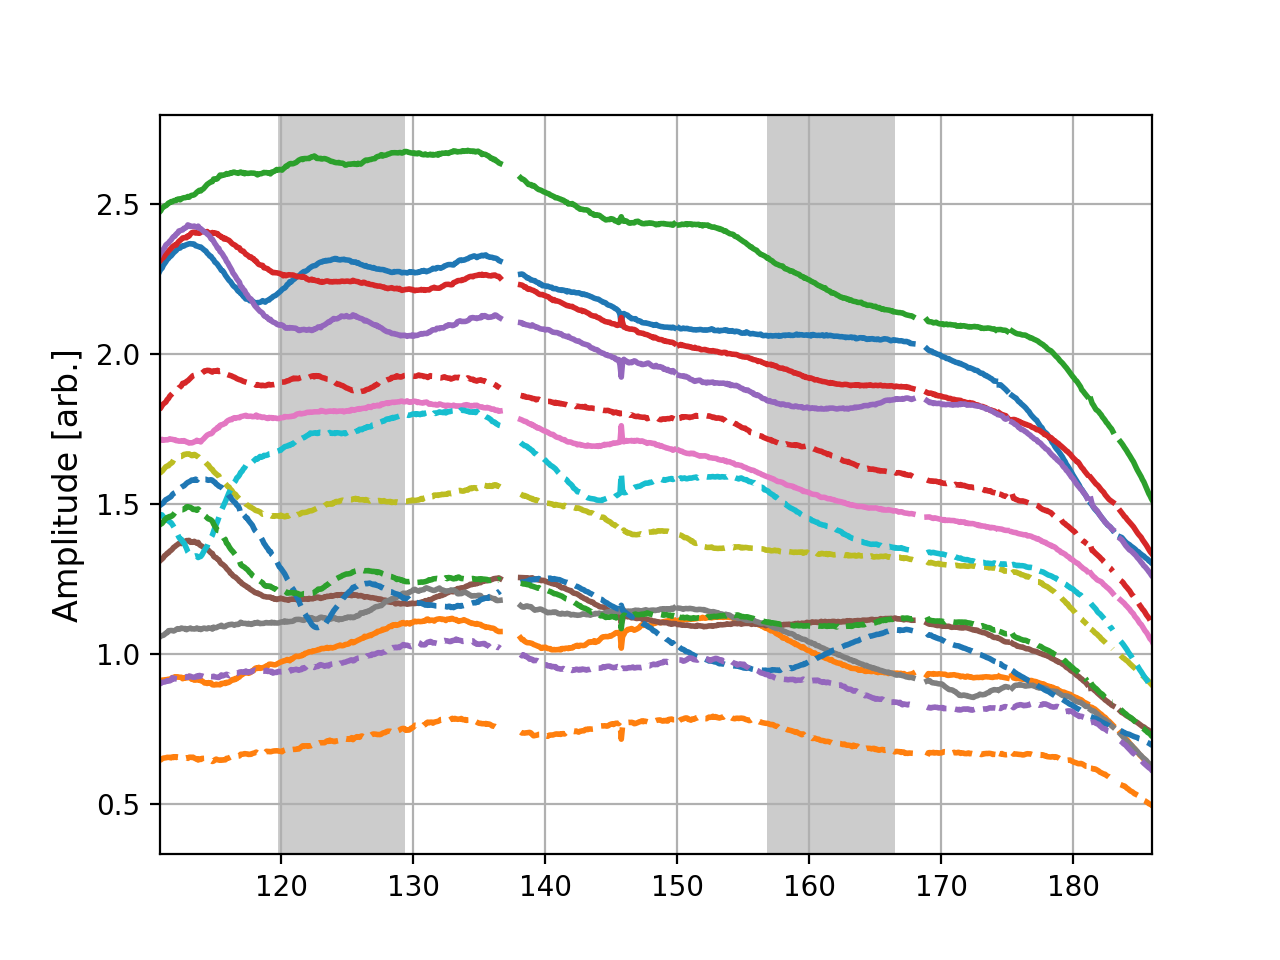
\includegraphics[scale=0.5]{chapters/eor_window_HERA/figures/h19_2457458_abs_smallzoom_nolegend.png}
\caption[Bandpass solutions for the North-South dipole orientation obtained for the functioning antennae in the array on JD 2457548.]{Bandpass solutions for the North-South dipole orientation obtained for the functioning antennae in the array on JD 2457548. Differences in line color and style is merely to distinguish different antennae. Shaded regions indicate the effective sub-bands used for power spectrum analysis.}
\label{fig:hera19_bandpass}
\end{figure}

The complex gain solutions were subsequently applied to the {\sc miriad} files. Figure~\ref{fig:hera19_phasecal} shows the effect of calibration on the visibilities of three nominally redundantly-spaced baselines. Shown in that figure are the phases of three $V^{nn}$ visibilities from 14.7\,m baselines before and after calibration. There were no shared antennae between the visibilities shown. The qualitative agreement is obvious, providing a consistency check on the solutions. We did not attempt to calibrate \textit{D}-terms in this work.

\begin{figure}
\centering
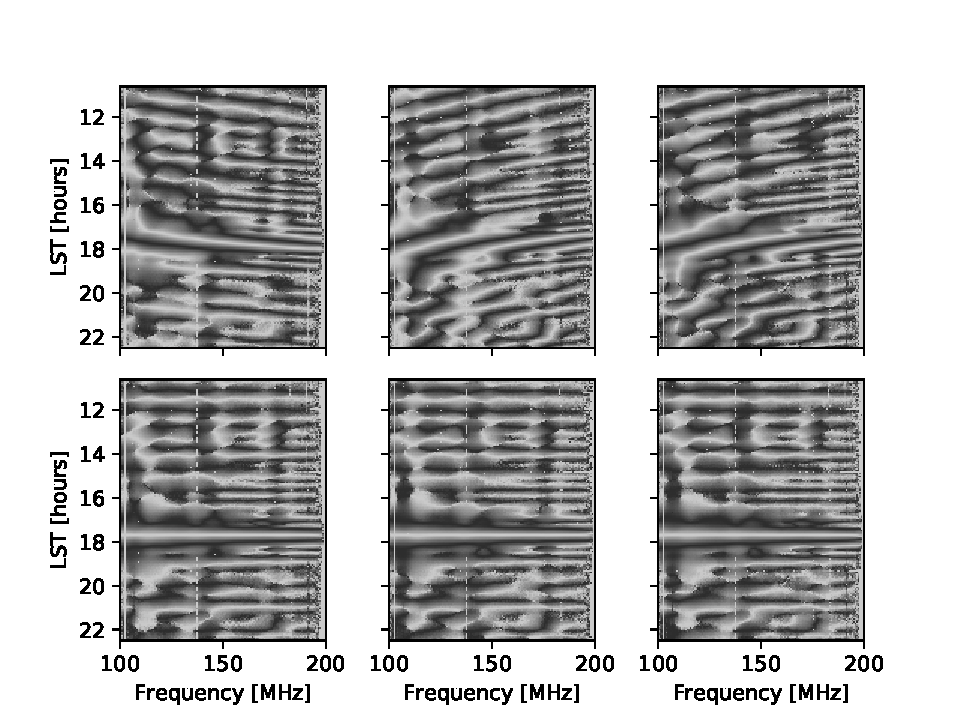
\includegraphics[width=0.9\textwidth]{chapters/eor_window_HERA/figures/phases_pre_post_abscal_h19_cyclic_grey.pdf}
\caption[The effect of calibration on the phases of visibilities from three redundantly-spaced 14.7\,m baselines.]{The effect of calibration on the phases of visibilities from three redundantly-spaced 14.7\,m baselines; \textit{nn} polarization. The color scale is cyclic; black is $\pm\pi/2$ and white is 0 and $\pm\pi$. \textit{Above}: before calibration; \textit{below}: after calibration. A simple sky model was sufficient to enforce redundancy for redundant baselines.}
\label{fig:hera19_phasecal}
\end{figure}


%This limited our interpretive power, which we discuss in Section~\ref{sec:results}.

We down-selected to two relatively RFI-free 20 MHz sub-bands (Figure~\ref{fig:hera19_rfi}); 115 to 135 MHz and 152 to 172 MHz, henceforth referred to the ``low band'' and the ``high band''. As we discuss in Section~\ref{subsec:hera19_pspec}, these bands were multiplied by a Blackman-Harris window, centered on their central frequencies, before Fourier transforming in order to minimize side-lobes. This windowing lead to an noise-effective bandwidth of 10 MHz, appropriate for EoR analyses since the {\sc hi} signal is to a reasonable approximation coeval over the corresponding redshift range \citep{Furlanetto.06}.

Pseudo-Stokes visibilities were formed from the instrumental polarizations. These visibilities were then scaled to the appropriate amplitude using a model for the GC spectrum 

\begin{equation}
S_{\rm Sgr A^*}(\nu) \approx  3709 {\rm\, Jy} \times (\nu/408 {\rm \,MHz})^{-0.5}
\label{eq:freq_scale}
\end{equation}
drawn from the Global Sky Model \citep[GSM;][]{GSM.08,pygsm,GSM.17}. Note that the GSM is inherently $\sim 5\%$ uncertain at these frequencies. We note that this scaling is heavily resolution dependent; we are treating the Galactic Center as a point source when it is extended in reality. However, Section~\ref{sec:hera19_results} we show that we obtain sensible power levels for the foregrounds and noise, lending confidence to our overall scaling.

\subsection{Forming power spectra}
\label{subsec:hera19_pspec}

Power spectra were formed according to the method used in \cite{Pober.13} and \cite{Kohn.16}, which we briefly review here. All Fourier transforms were windowed using a Blackman-Harris window at the center of the sub-band, which minimized sidelobes. \cite{Parsons.12a} define the \textit{delay transform} as the Fourier transform of a visibility for baseline $ij$ and pseudo-Stokes parameter $P$ along the frequency axis

\begin{equation}
\tilde{V}_{ij}^{P}(\tau, t) = \int {\rm d}\nu \tilde{V}_{ij}^{P}(\nu, t)e^{2\pi i \nu \tau}.
\end{equation}

We note that using a Blackman-Harris window will induce a correlation between consecutive $\tau$ modes. The Fourier transform of the window function in frequency will be sharply peaked in the delay space, and can be ignored to some extent. Hence the self-correlation of $V_{ij}^{P}(\tau, t)$ can be used to define the power spectrum, although the small correlation of different $\tau$ modes could effect the variance of the power spectrum \citep{Parsons.14}.

The power at each delay-mode and baseline can be represented in terms of their respective Fourier components $k_{\parallel}$ and $k_{\perp}$ \citep{Parsons.12a, Nithya.15b}:
\begin{align*}
P(k_{\parallel},k_{\perp}) &\approx | \tilde{V}_{ij}^{P}(\tau) |^2 \frac{X^2 Y}{\Omega B} \left(\frac{c^2}{2k_B\nu^2}\right)^2 , \\\\
k_{\parallel} &= \frac{2\pi \nu_{\rm 21cm} H(z) %H_0 \sqrt{\Omega_m (1+z)^3 + \Omega_k (1+z)^2 + \Omega_{\Lambda}} 
}{c (1+z)^2}\tau, \\\\
k_{\perp} &= \frac{2\pi}{D(z) \lambda} b\\
\end{align*}
for: bandwidth $B$, angular area of the beam $\Omega$, $\nu_{\rm 21cm}\approx$1420 MHz, baseline length $b$, wavelength of observation $\lambda$, Hubble parameter $H(z)$, transverse comoving distance $D(z)$ and redshift-dependent scalars X and Y \citep{Parsons.12b}. Note that the angular area of the beam refers to the diagonal components of the Mueller matrices shown in Figure~\ref{fig:interferometry_Mab}. For further discussion of forming polarized power spectra in $k$-space, refer to \cite{Nunhokee.17}.

To avoid a noise-bias when forming the $ |\tilde{V}_{ij}^{P}(\tau, t) |^2$ term, we cross-multiplied consecutive integrations, rephasing the zenith angle of the latter to the former:

\begin{equation}
 | \tilde{V}_{ij}^{P}(\tau, t) |^2 \approx | \tilde{V}_{ij}^{P}(\tau, t) \times \tilde{V}_{ij}^{P}(\tau, t+\Delta t)e^{i\theta_{ij,\rm zen}(\Delta t)}|
\end{equation}
where $\theta_{ij,\rm zen}(\Delta t)$ was the appropriate phasing for baseline $ij$ and $\Delta t = 10.7$ seconds.

Pseudo-stokes power spectra were formed for each pair of integrations, for every baseline. After forming power spectra, baselines of identical lengths were averaged together. Appealing to cosmological isotropy, baselines of the same length but different orientation should be sampling the same cosmological structure. These 2D power spectra were averaged over our 8 days of observations. Note that all averaging was performed after forming power spectra; this incoherent averaging was non-optimal from a signal-to-noise perspective outside the wedge, slightly reducing our sensitivity in the EoR window. However, the intention of this investigation was not a deep integration on noise; we were more interested in the polarized response of the instrument. As such, the power spectra presented in the Section below should be interpreted as approximate.

\section{Results \& Discussion}
\label{sec:hera19_results}

%We formed two-dimensional power spectra (that is, power gridded into the ($k_{\perp}$, $k_{\parallel}$) plane) for each JD and pseudo-Stokes parameter, and averaged those power spectra together. Averaging in the squared power between days is non-optimal in terms of attempting an EoR detection, but we were concerned with foregrounds in $k$-space for this study, and it reduced the variance of foreground power within the ``pitchfork" region.

Power spectra are shown for the high and low bands in Figure~\ref{fig:hera19_pitchforks_highband} and Figure~\ref{fig:hera19_pitchforks_lowband}, respectively, where white dotted lines mark the boundary of the EoR window on the 2D plots.  The same data are presented in middle and lower panels, with the latter overlaid as lines to emphasize common features of the power spectra with respect to baseline length. 

Theoretical noise levels for the high and low bands were between 
$P_{\rm noise}(k)\approx$ 1.7$\times$10$^8$ \,mK$^2$Mpc$^3$h$^{-3}$ -- 3.4$\times$10$^9$ \,mK$^2$Mpc$^3$h$^{-3}$ in the high band, and 2.3$\times$10$^8$ \,mK$^2$Mpc$^3$h$^{-3}$ -- 6.1$\times$10$^9$ \,mK$^2$Mpc$^3$h$^{-3}$ in the low band. These estimates used a temperature model of the sky

\begin{equation}
T_{\rm sky} = 180\,{\rm K} \left(\frac{\nu}{180\,{\rm MHz}}\right)^{-2.55},
\end{equation}
assumed receiver temperatures of 300\,K and 600\,K for the high band and low band, respectively \citep[][also see the public HERA Memo \# 16]{deBoer.17}. They were calculated according to the formalism for noise power spectra in \cite{Parsons.12a}, with the inclusion of a baseline-number dependence (to account for different occupancies in each $k_{\perp}$ bin).
The estimates were roughly corroborated by our observations (see Figure~\ref{fig:hera19_highband_cuts_per_day}). We observe excess noise on the shortest baselines (also obvious in the lower panels of Figures~\ref{fig:hera19_pitchforks_highband} and \ref{fig:hera19_pitchforks_lowband}). 

\subsection{General features of the power spectra}
\label{subsec:general_features}
The most striking feature of these power spectra is the degree of foreground isolation achieved in all pseudo-Stokes parameters. In similar studies of 2D polarized power spectra, both PAPER \citep{Kohn.16} and LOFAR \citep{Asad.17} measurements found ``filled'' regions of Fourier space out to the edge of the EoR window (in the delay-spectrum paradigm, this corresponds to the horizon; zenith angle $\pm$90$^{\circ}$), with some supra-horizon leakage \citep{Pober.13} into the EoR window itself. The power spectra in Figures~\ref{fig:hera19_pitchforks_highband} and \ref{fig:hera19_pitchforks_lowband} show no such behavior; all foreground emission appears to be contained within a narrow region around $k_{\parallel}=0$ h/Mpc. This behavior was predicted for an array of HERA-like dishes by \citealt{Nithya.15b} (although that study only concentrated on the Stokes I component). 

Power at horizon delays, as predicted by \cite{Nithya.15b} and \cite{Neben.16}, was not observed. This was likely a resolution effect. To resolve horizon-delay power, one would need to sample many periods of $\tau_h=b/c$, where $b$ is the magnitude of the baseline vector. The maximum length baseline in the HERA-19 array was 58.4\,m, corresponding to a $\sim$5 MHz period: barely sampled by the 10\,MHz windows we use in this study. The lack of horizon power is corroborated by the simulations of the HERA delay response in \cite{Ewall-Wice.16.HERA_Dish} and \cite{Thyagarajan.16}, although those studies used a different windowing function for the delay transform. Their simulations also predict a high degree of foreground isolation: the presence of noise in our data of course meant that we do not realize the 11 dex of isolation that can be achieved in simulation, but the $\sim$8 dex we do see, without any foreground subtraction and a simple calibration, speaks to the power of HERA's future capabilities.

\begin{figure*}[h]
\centering
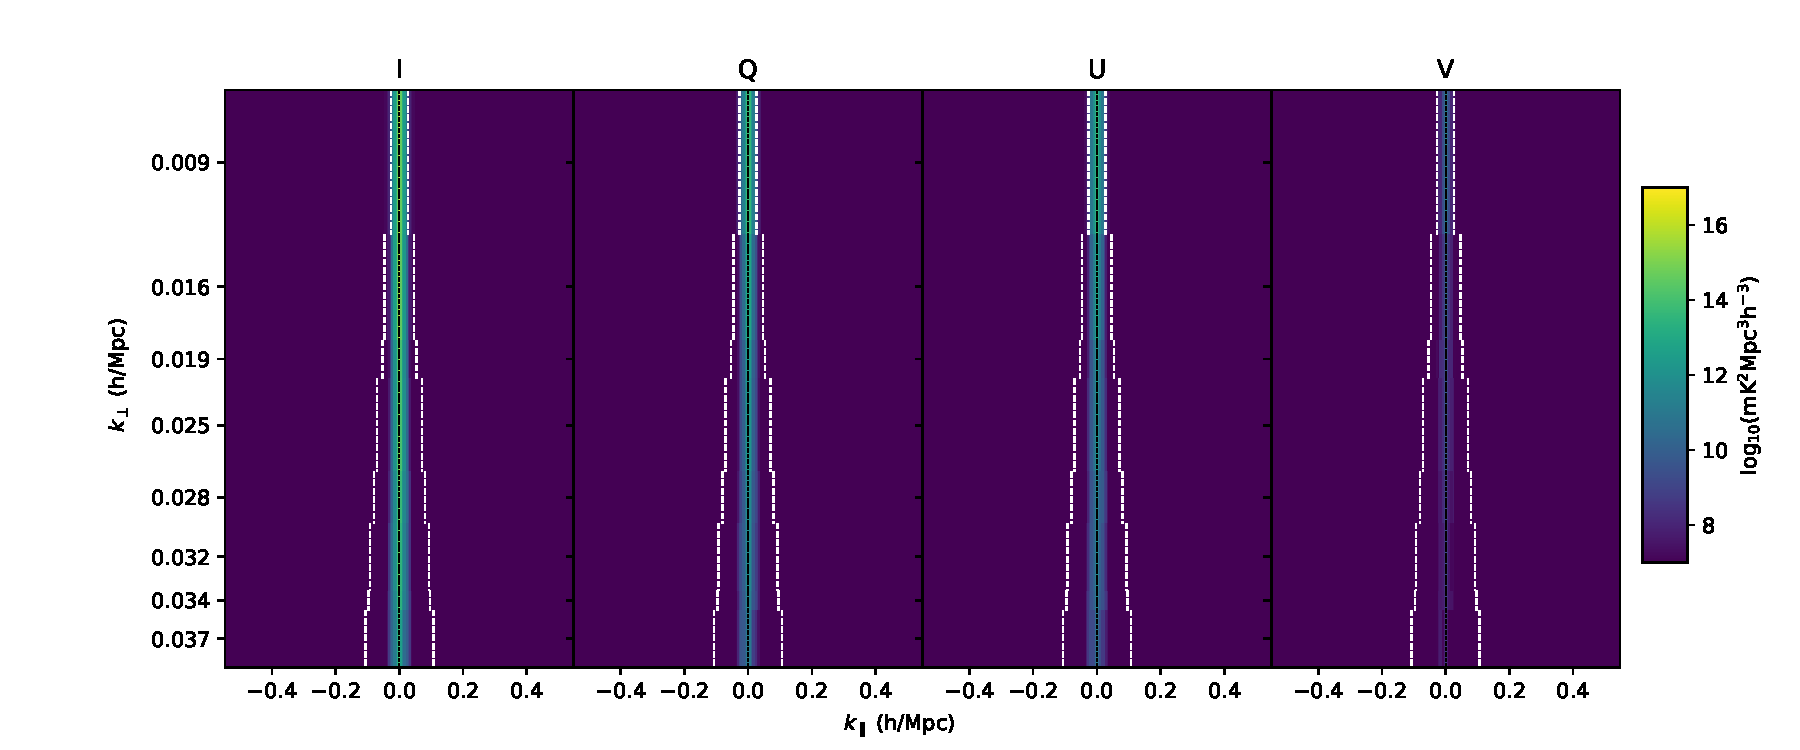
\includegraphics[scale=0.45]{chapters/eor_window_HERA/figures/timeavg_SIM_high.pdf}
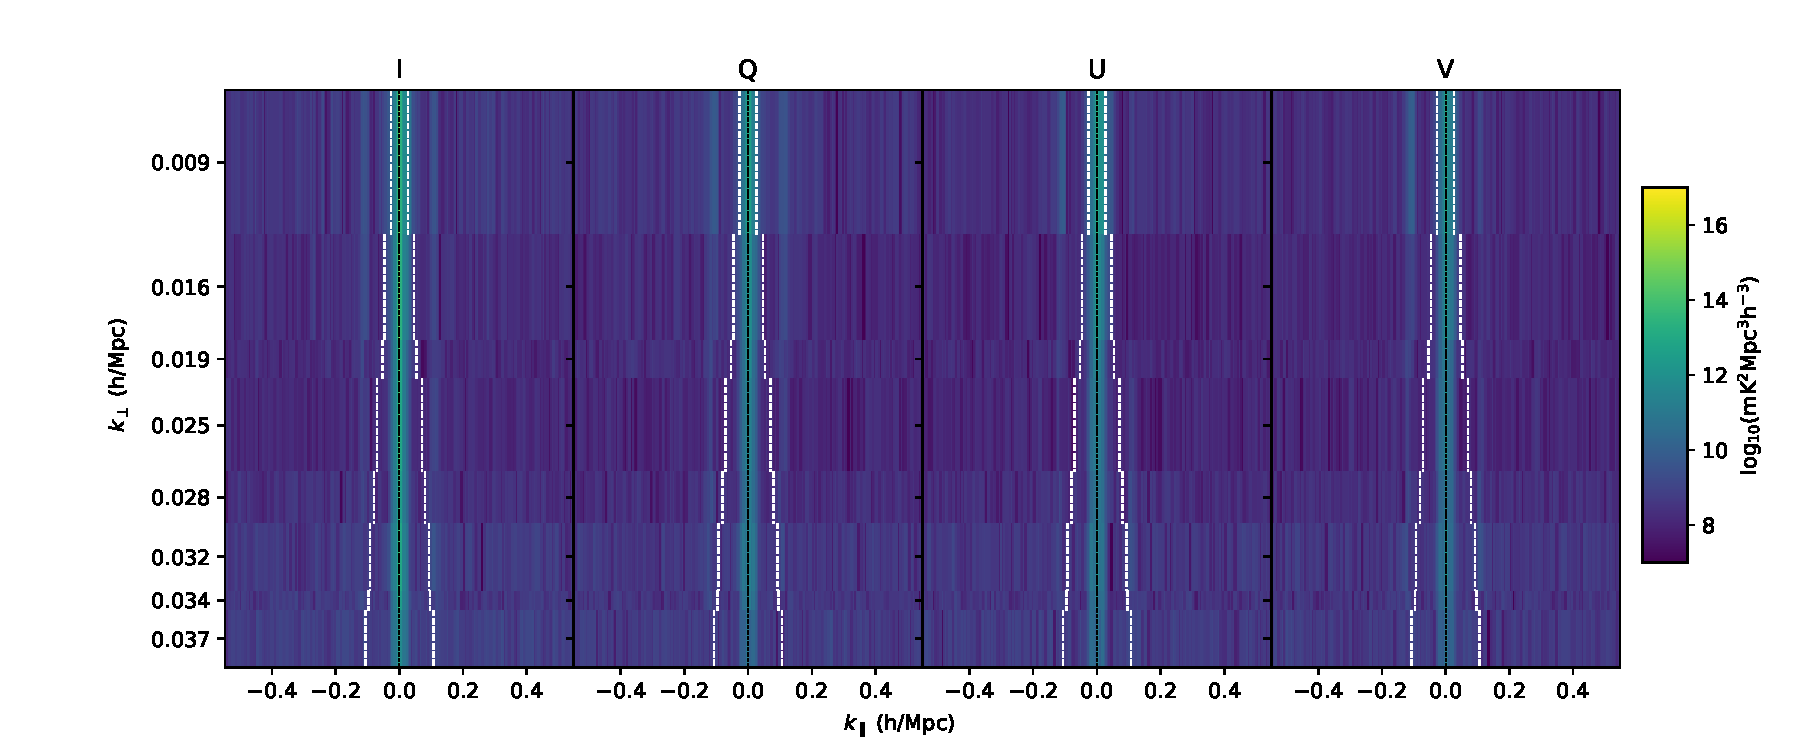
\includegraphics[scale=0.45]{chapters/eor_window_HERA/figures/timeavg_high.pdf}
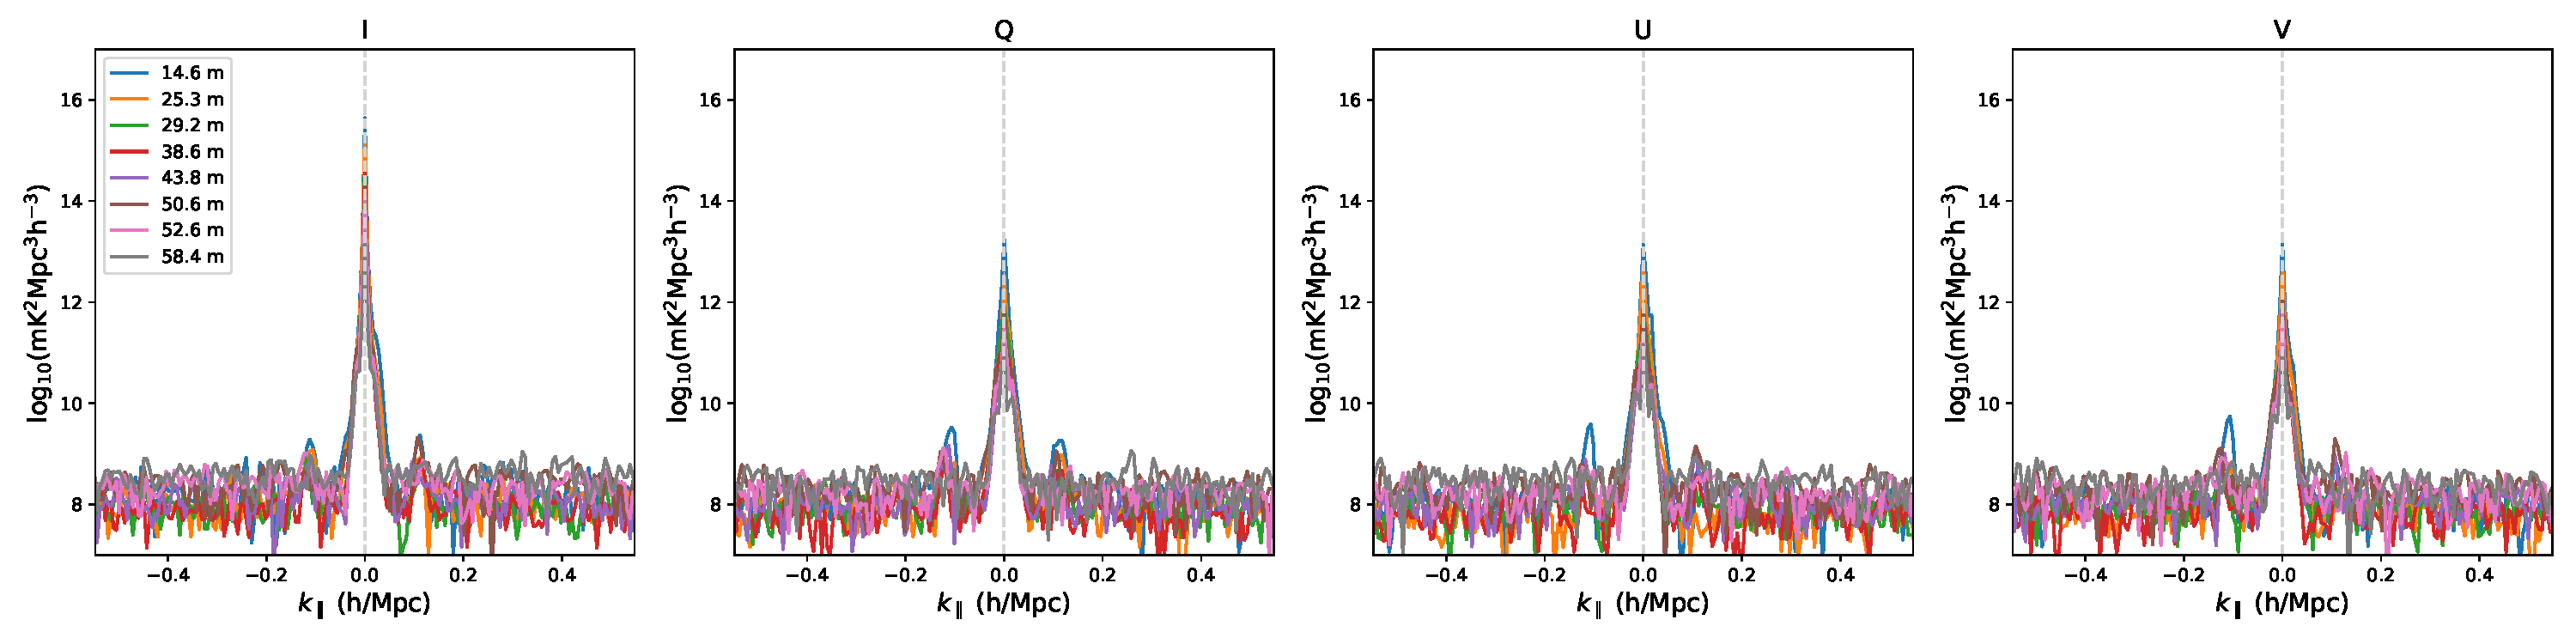
\includegraphics[scale=0.3]{chapters/eor_window_HERA/figures/timeavg_1d_high.pdf}
\caption[Power spectrum results from the high-band (157--167 MHz).]{Results from the high-band (157--167 MHz). White dotted lines indicate the boundary of the pitchfork and the EoR window. A black dotted line indicates the $k_{\parallel}=0$\,h/Mpc line. \textit{Top}: Simulated power spectra in Stokes I, Q, U and V, following the formalism in Section~\ref{sec:hera19_leak} -- no polarized sky model was used, so power in Stokes Q, U and V was only due to direction-dependent leakage from Stokes I. No instrumental noise was included in the simulation. \textit{Middle}: Eight-day average power spectra from data. \textit{Bottom}: The same data as shown in the middle panel, but with each baseline length overlaid on one another to allow shared features to be more easily identified.}
\label{fig:hera19_pitchforks_highband}
\end{figure*}

\begin{figure*}[h]
\centering
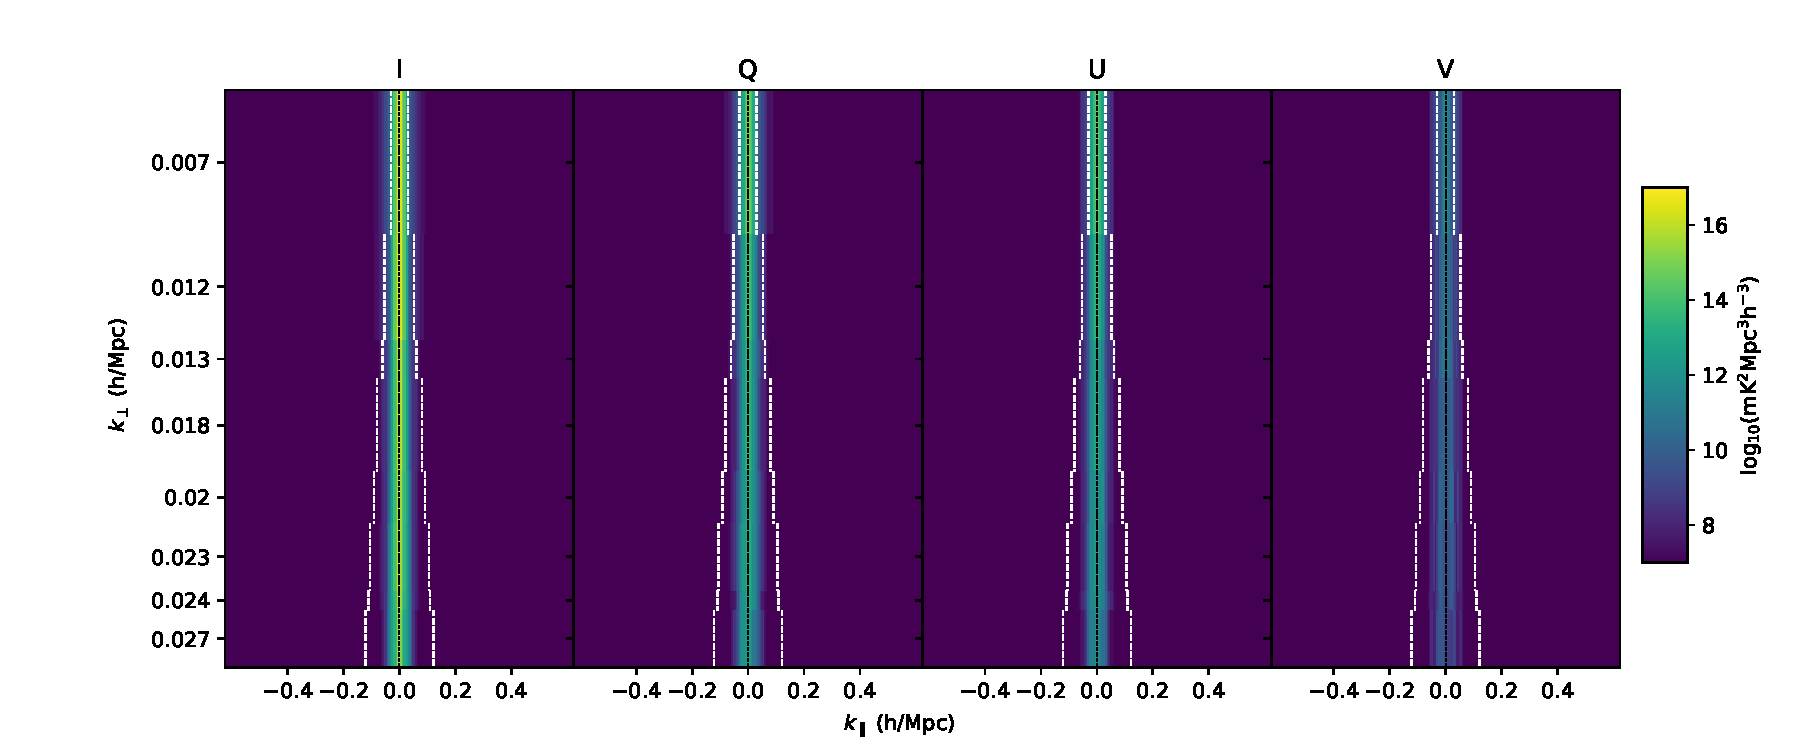
\includegraphics[scale=0.45]{chapters/eor_window_HERA/figures/timeavg_SIM_low.pdf}
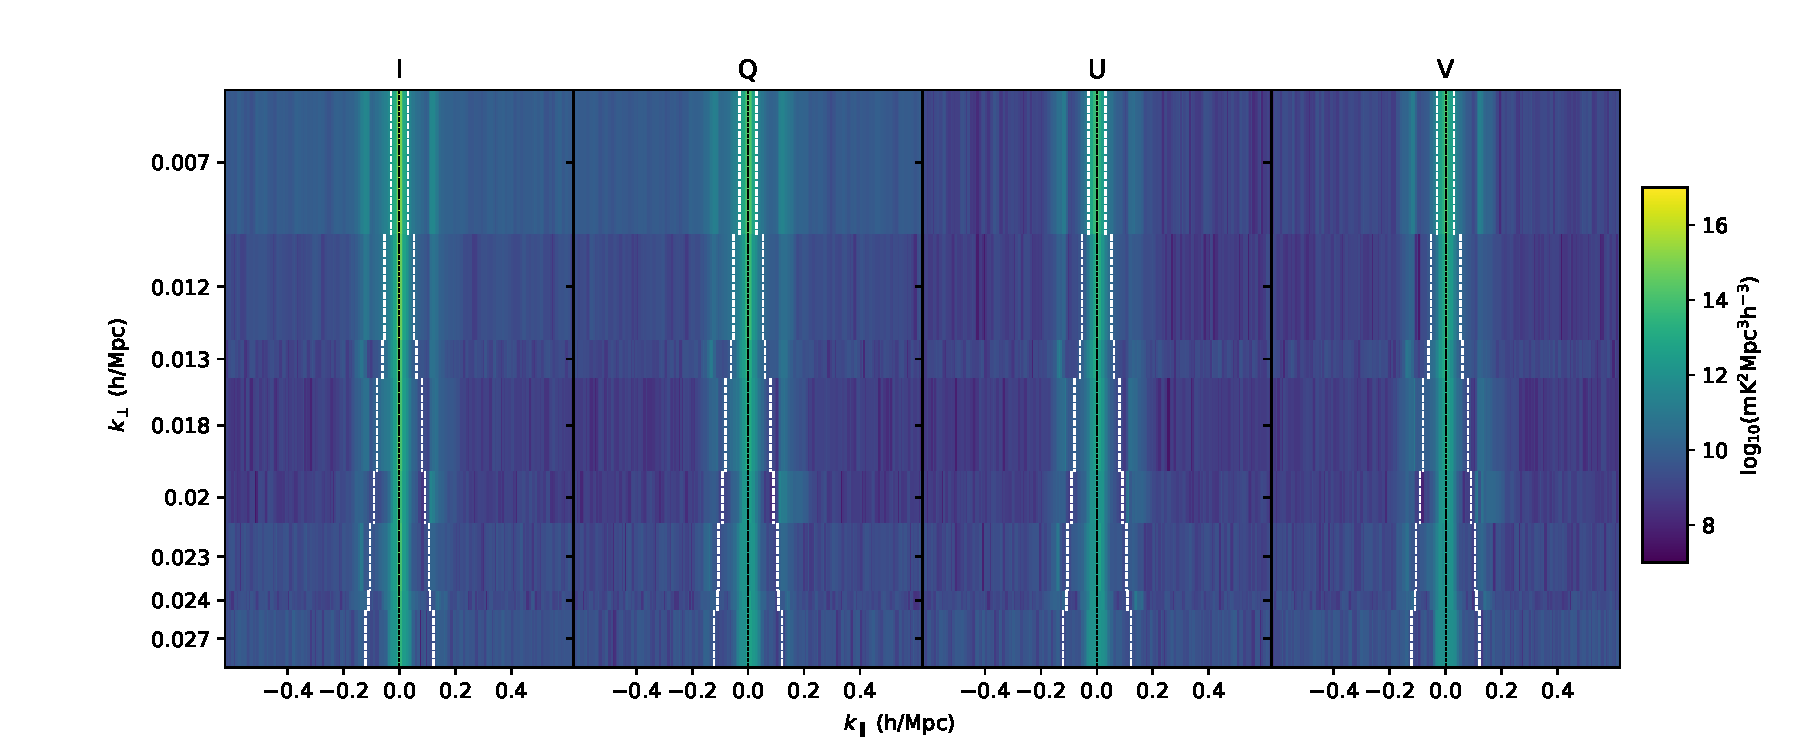
\includegraphics[scale=0.45]{chapters/eor_window_HERA/figures/timeavg_low.pdf}
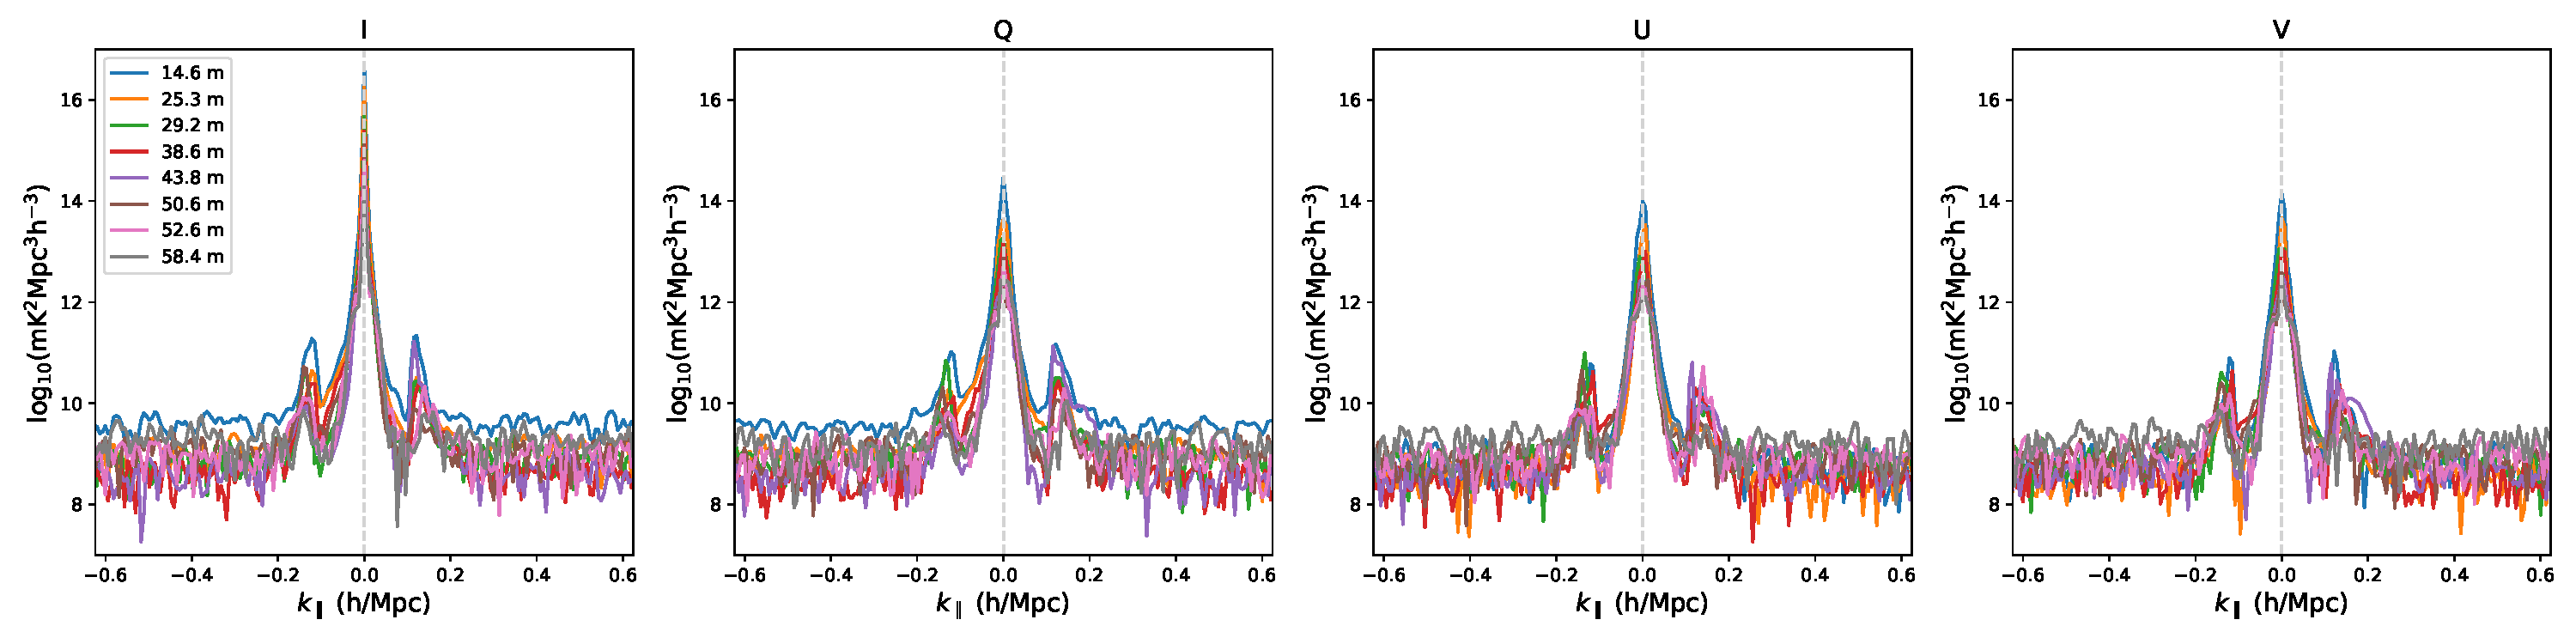
\includegraphics[scale=0.3]{chapters/eor_window_HERA/figures/timeavg_1d_low.pdf}
\caption[Power spectrum results from the low-band (120--130 MHz).]{Results from the low-band (120--130 MHz), arranged in the same format as Figure~\ref{fig:hera19_pitchforks_highband}.}
\label{fig:hera19_pitchforks_lowband}
\end{figure*}

Visible in the observational data, but not in the simulation, is an excess of power at $k_{\parallel}=0.04$\,h/Mpc, corresponding to a delay of 100\,ns, which is independent of baseline length. This suggests that its origins are in the HERA signal chain. There are 15\,m coaxial cables at one stage of the signal chain from the HERA dishes to the correlator\footnote{This stage of the signal chain is only present in the commissioning array. Future HERA build-outs will transition to a different architecture \citep{deBoer.17}.}. In the limit of little delay induced by the cable and our limited delay resolution, a reflection along this stage of the signal chain would produce an alias of the foreground signal at a $\tau \approx 100$\,ns \citep{Beardsley.16, Ewall-Wice.EoX}.
\clearpage
\subsection{Day-to-day variability}

The foreground and EoR window power levels appeared to be relatively stable between days, with variation most likely due to the incomplete sky model used for gain calibration. Figure~\ref{fig:hera19_highband_cuts_per_day} shows power as a function of baseline length for $k_{\parallel}=0$ h/Mpc (solid lines) and $k_{\parallel}=0.2$ h/Mpc (dot-dashed lines). Deviations from the mean at $k_{\parallel}=0$ h/Mpc may be a limitation imposed by our simplistic sky model. Since the noise levels in the EoR window region remained noise-like throughout our observations, the uncertainty in the absolute gain scale did not have a large impact on our largely-diagnostic investigation.

\begin{figure}
\centering
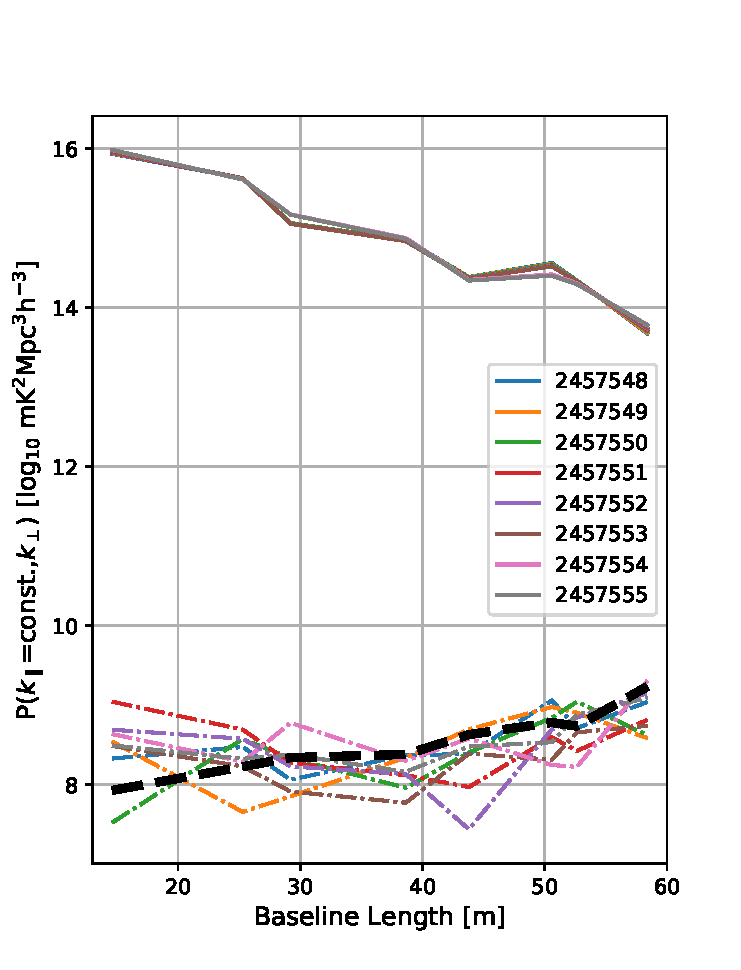
\includegraphics[scale=0.5]{chapters/eor_window_HERA/figures/highband_by_day.pdf}
\caption[High band power as a function of baseline length for the center of the pitchfork ($k_{\parallel}=0$ h/Mpc) and in the EoR window ($k_{\parallel}=0.2$ h/Mpc) for each JD of observation. ]{High band power as a function of baseline length for the center of the pitchfork ($k_{\parallel}=0$ h/Mpc; solid lines) and in the EoR window ($k_{\parallel}=0.2$ h/Mpc; dot-dashed lines) for each JD of observation. The black dashed line represents the approximate noise power assuming a receiver temperature of 300\,K. A very similar relationship is shown in the low band, but with a higher noise floor, which is consistent with system temperature as a function of frequency. The noise level climbs with baseline length as the compact nature of the array gives more short baselines to average-over in a given $(k_{\parallel},k_{\perp})$ bin than longer ones.}
\label{fig:hera19_highband_cuts_per_day}
\end{figure}

\subsection{Polarimetric results}
\label{subsec:polarimetric_results}

Figures~\ref{fig:hera19_pitchforks_highband} and~\ref{fig:hera19_pitchforks_lowband} qualitatively illustrate that the simulations described in Section~\ref{sec:hera19_leak} reproduced the main features of the observed power spectra. The simulations were run only with a Stokes I sky component and no simulated calibration errors, so the only signal in the polarized power spectra was from wide-field beam leakage (Figure~\ref{fig:interferometry_Mab}). An example comparison between simulation and observation in the image plane is shown in Figure~\ref{fig:hera19_GCimage}.

In Figure~\ref{fig:hera19_bl0_cuts_vs_sim} we show the power levels observed on the shortest baseline (14.7\,m) compared to our simulations for each band. The simulations used an unpolarized diffuse sky model \citep[the most recent version of the GSM;][]{GSM.17}, which should be accurate at the scales probed by a 14.7\,m baseline. Inset panels zoom-in on the region around $k_{\parallel}=0$\,h/Mpc, where most of the foreground power was concentrated.
We saw that the simulations reproduced $\sim75\%$ of the foreground power observed in pseudo-Stokes I in the high band, and over-predicted foreground power by $\sim35\%$ in the low band. This could have been due to unrealistic frequency scaling of the diffuse foregrounds in the GSM. 

For pseudo-Stokes Q and U, the simulations accounted for $\sim 60-75\%$ of power seen within the pitchfork region, suggesting that most of the power seen in these power spectra, at least for the shortest baselines, can be mostly attributed to direction-dependent leakage effects. As noted in Section~\ref{sec:hera19_leak}, residual gain and phase errors are able to leak a fraction of pseudo-Stokes I into Q and U, but some fraction of the observed power ($\leqslant 25\%$) may have been due to linearly polarized foregrounds. This is corroborated by residual power close to the location of the Galactic Center, and increased power over the sky, in the observed pseudo-Stokes Q and U skies compared to the simulated ones in Figure~\ref{fig:hera19_GCimage}. As the Galactic Center is the highest-amplitude source of power, we expect residual gain errors to be most obvious in the same position as it is in the pseudo-Stokes I image. Such an excess is present in the observed pseudo-Stokes Q and U images, but absent in the simulated ones -- pointing to direction-independent gain errors being present. However, the simulated pseudo-Stokes Q and U images contain only direction-dependent leakage from Stokes I. Since they reproduce most of the features seen in the observed data, pseudo-Stokes Q and U are clearly dominated by direction dependent leakage.

\cite{Lenc.16} observed linearly polarized emission from diffuse structure with $\sim 1.6 - 4.5\%$ fractional polarization at 150\,MHz, corresponding to power levels of $\sim10^5$ mK$^2$Mpc$^3$h$^{-3}$. This power level is similar to expected EoR power levels \citep[e.g.][]{Lidz.07, Moore.13, Nunhokee.17}; a detection of a power spectrum of polarized galactic synchrotron will require much deeper integrations.

\begin{figure*}
\centering
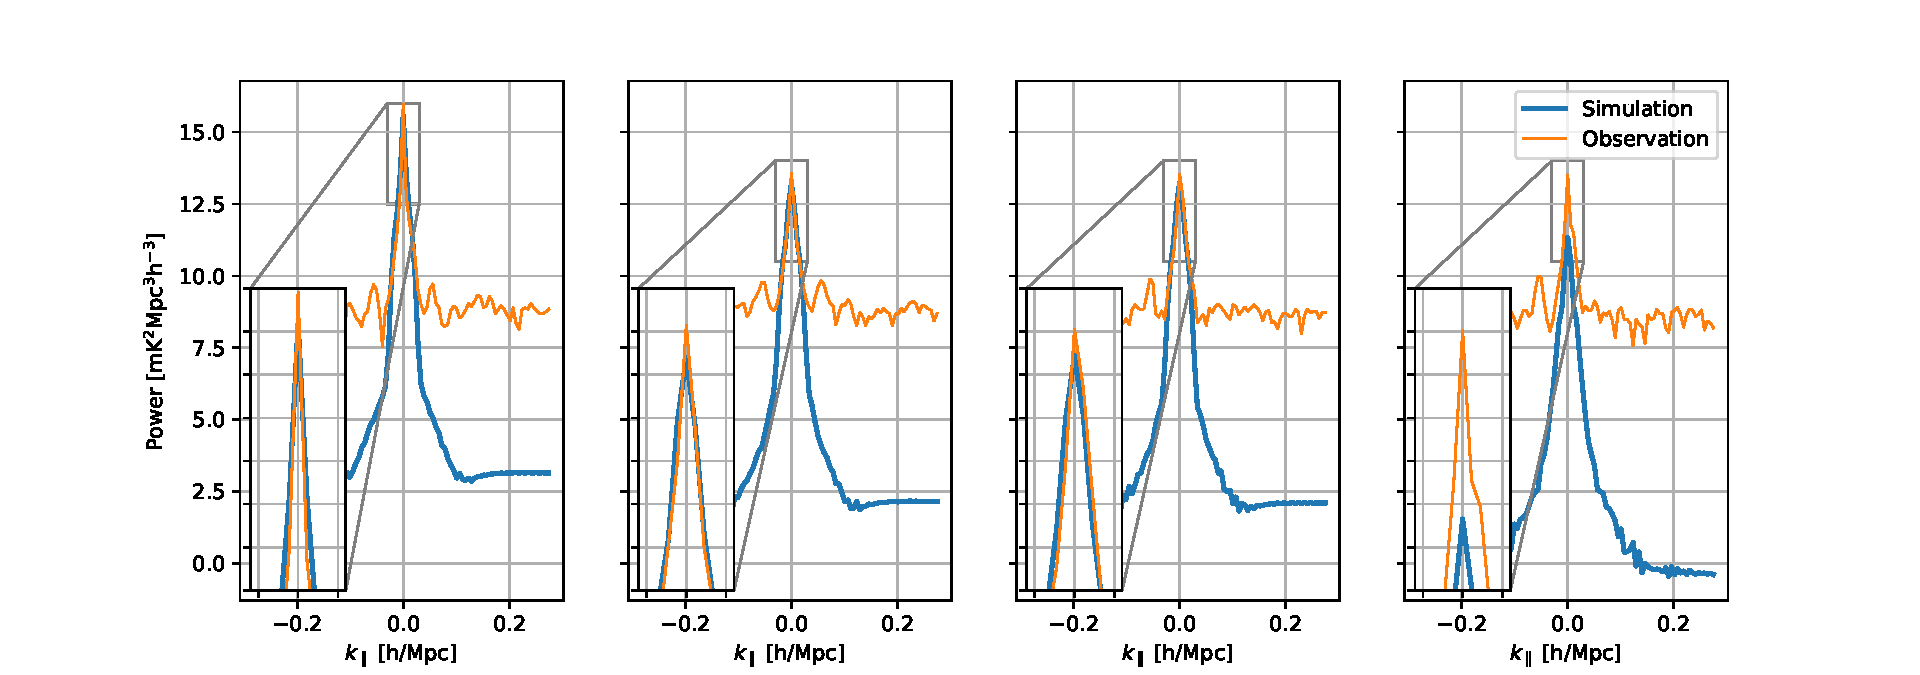
\includegraphics[width=0.9\textwidth]{chapters/eor_window_HERA/figures/highband_bl0_4pol_with_zoom.pdf}\\
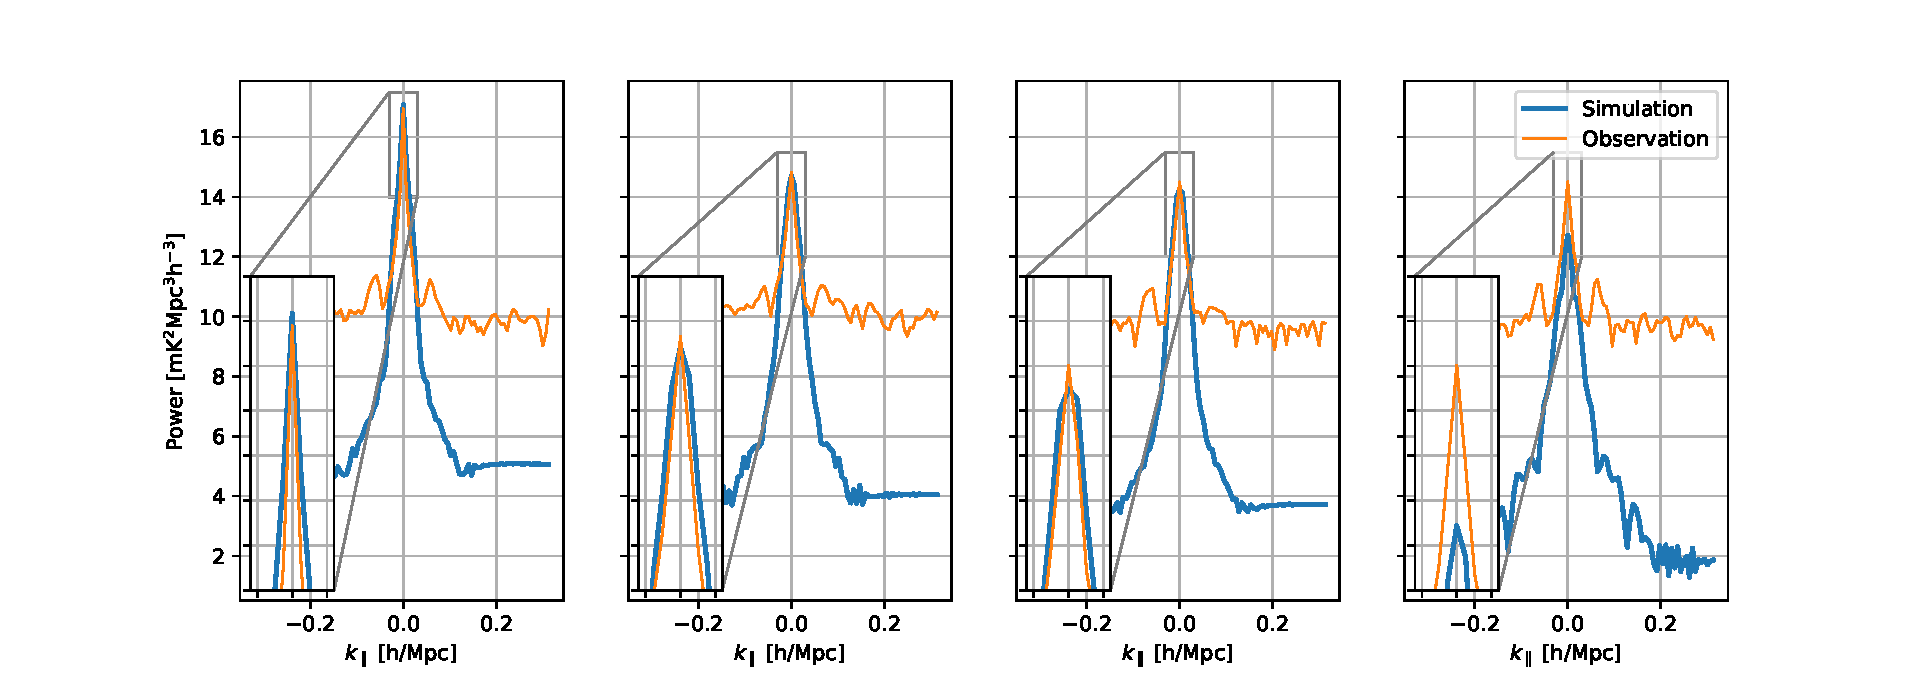
\includegraphics[width=0.9\textwidth]{chapters/eor_window_HERA/figures/lowband_bl0_4pol_with_zoom.pdf}
\caption[Simulated and observed power as a function of $k_{\parallel}$ for the shortest baseline (14.7\,m).]{Simulated and observed power as a function of $k_{\parallel}$ for the shortest baseline (14.7\,m). \textit{Right to left}: pseudo-Stokes I, Q, U and V; \textit{above}: the high band; \textit{below}: the low band. The simulations were noiseless and used an unpolarized sky model. Inset panels zoom-in on the peak region. They capture the foreground power levels in pseudo-Stokes I, Q and U, suggesting all power in Q and U is due to leakage from Stokes I. The power level in V is highly discrepant, however, suggesting some sort of beam-independent instrumental leakage.}
\label{fig:hera19_bl0_cuts_vs_sim}
\end{figure*}

The observed pseudo-Stokes V power spectrum was more poorly modelled by our simulation. In both bands we observed $\sim$20 dB more power in pseudo-Stokes V at $k_{\parallel}=0$\,h/Mpc than predicted by our simulations. The peak power observed in pseudo-Stokes V was roughly 0.1\% of the peak power observed in pseudo-Stokes I. Likewise in the sky images shown in Figure~\ref{fig:hera19_GCimage}, there is little pseudo-Stokes V power in the simulated images, compared to observation. This suggests that most or all of the power in pseudo-Stokes V is due to direction independent leakage. While the leakage appears localized in Figure~\ref{fig:hera19_GCimage}, we see in Figure~\ref{fig:hera19_bl0_cuts_vs_sim} that it is statistically similar to pseudo-Stokes Q and U in power.
Since $D$-terms cause direction-independent leakage from pseudo-Stokes I to pseudo-Stokes V, the excess power we observed could be interpreted as an approximate $D$-term level of $\sim$1\% \citep{TMS}. This is similar to $D$-term levels from other low frequency instruments such as MWA-32, which was found to have $\sim$2\% $D$-terms (G. Bernardi, private communication). 
The under-prediction of pseudo-Stokes V from the simulation could, of course, also be due to some unmodelled direction-dependent instrumental effect.

To understand which effect, if either, is dominant, a precise $D$-term calibration of HERA is required. This effort is underway with data taken with bright polarized point sources in transit, and will be presented in future work. Another potential cause of the discrepancy could have been that our simulations under-predicted Stokes V power, due to lack of accounting for some variety of instrumental circular polarization.

In Section~\ref{subsec:general_features} we noted the presence of excess power at $k_{\parallel}=\pm 0.04$\,h/Mpc ($\pm$100\,ns) that was independent of baseline length, suggesting that it was due to a reflection along 15\,m cables. Figure~\ref{fig:hera19_bl0_cuts_vs_sim} shows that power at this delay is not consistent between polarizations. Stokes U and V power only exhibited excess signal at -100\,ns in the high band, and in the low band, it was only Stokes U that did not exhibit that excess at +100\,ns. This may be a clue about the polarization state of cable reflections, perhaps as a function of frequency, but we defer this to future work -- noting it as a point of interest here.

\section{Conclusions}
\label{sec:hera19_conc}

In this work we have presented polarized power spectra from the HERA-19 commissioning array. With modest calibration, HERA is able isolate total intensity and polarized foregrounds to within the ``pitchfork'' region of \textit{k}-space, as predicted by \cite{Nithya.15b}, lending confidence to its future performance as an instrument capable of both detecting and characterizing the EoR power spectrum. Of course, the array used in this study had just 19 antennae, 15 of which were used for analysis -- future build-outs of HERA with up to 350 antennae will require strong quality-assurance efforts.

Simulations of the polarized response of the instrument, mapped into the same Fourier space as the data, suggest that most or all of the polarized power observed in pseudo-Stokes Q and U power spectra is due to direction-dependent beam leakage from pseudo-Stokes I. Residual gain and phase errors could account for the rest of the power, but some fraction of the total ($\leqslant 25\%$) may be due to linearly polarized foregrounds. Excess power in pseudo-Stokes V may be due to $D$-terms at the 1\% level, but a full image-based calibration with a polarized point source is required to confirm this. The general accuracy of our simulations suggests current modelling of the complex HERA beam is accurate.